\begin{frame}[t,fragile]{Ausgangspunkt}
\begin{itemize}
\item Funktionalität eines Moduls musste verändert werden
\begin{itemize}
\item Bugfixing
\item neue Features
\item bessere Tests
\end{itemize}
\item Codequalität war unterirdisch (sowohl messbar als auch erfahrbar)
\end{itemize}

$\Longrightarrow$ Wir durften einen Umbau vornehmen
\end{frame}

\begin{frame}[t,fragile]{Vorhandene Codestruktur}
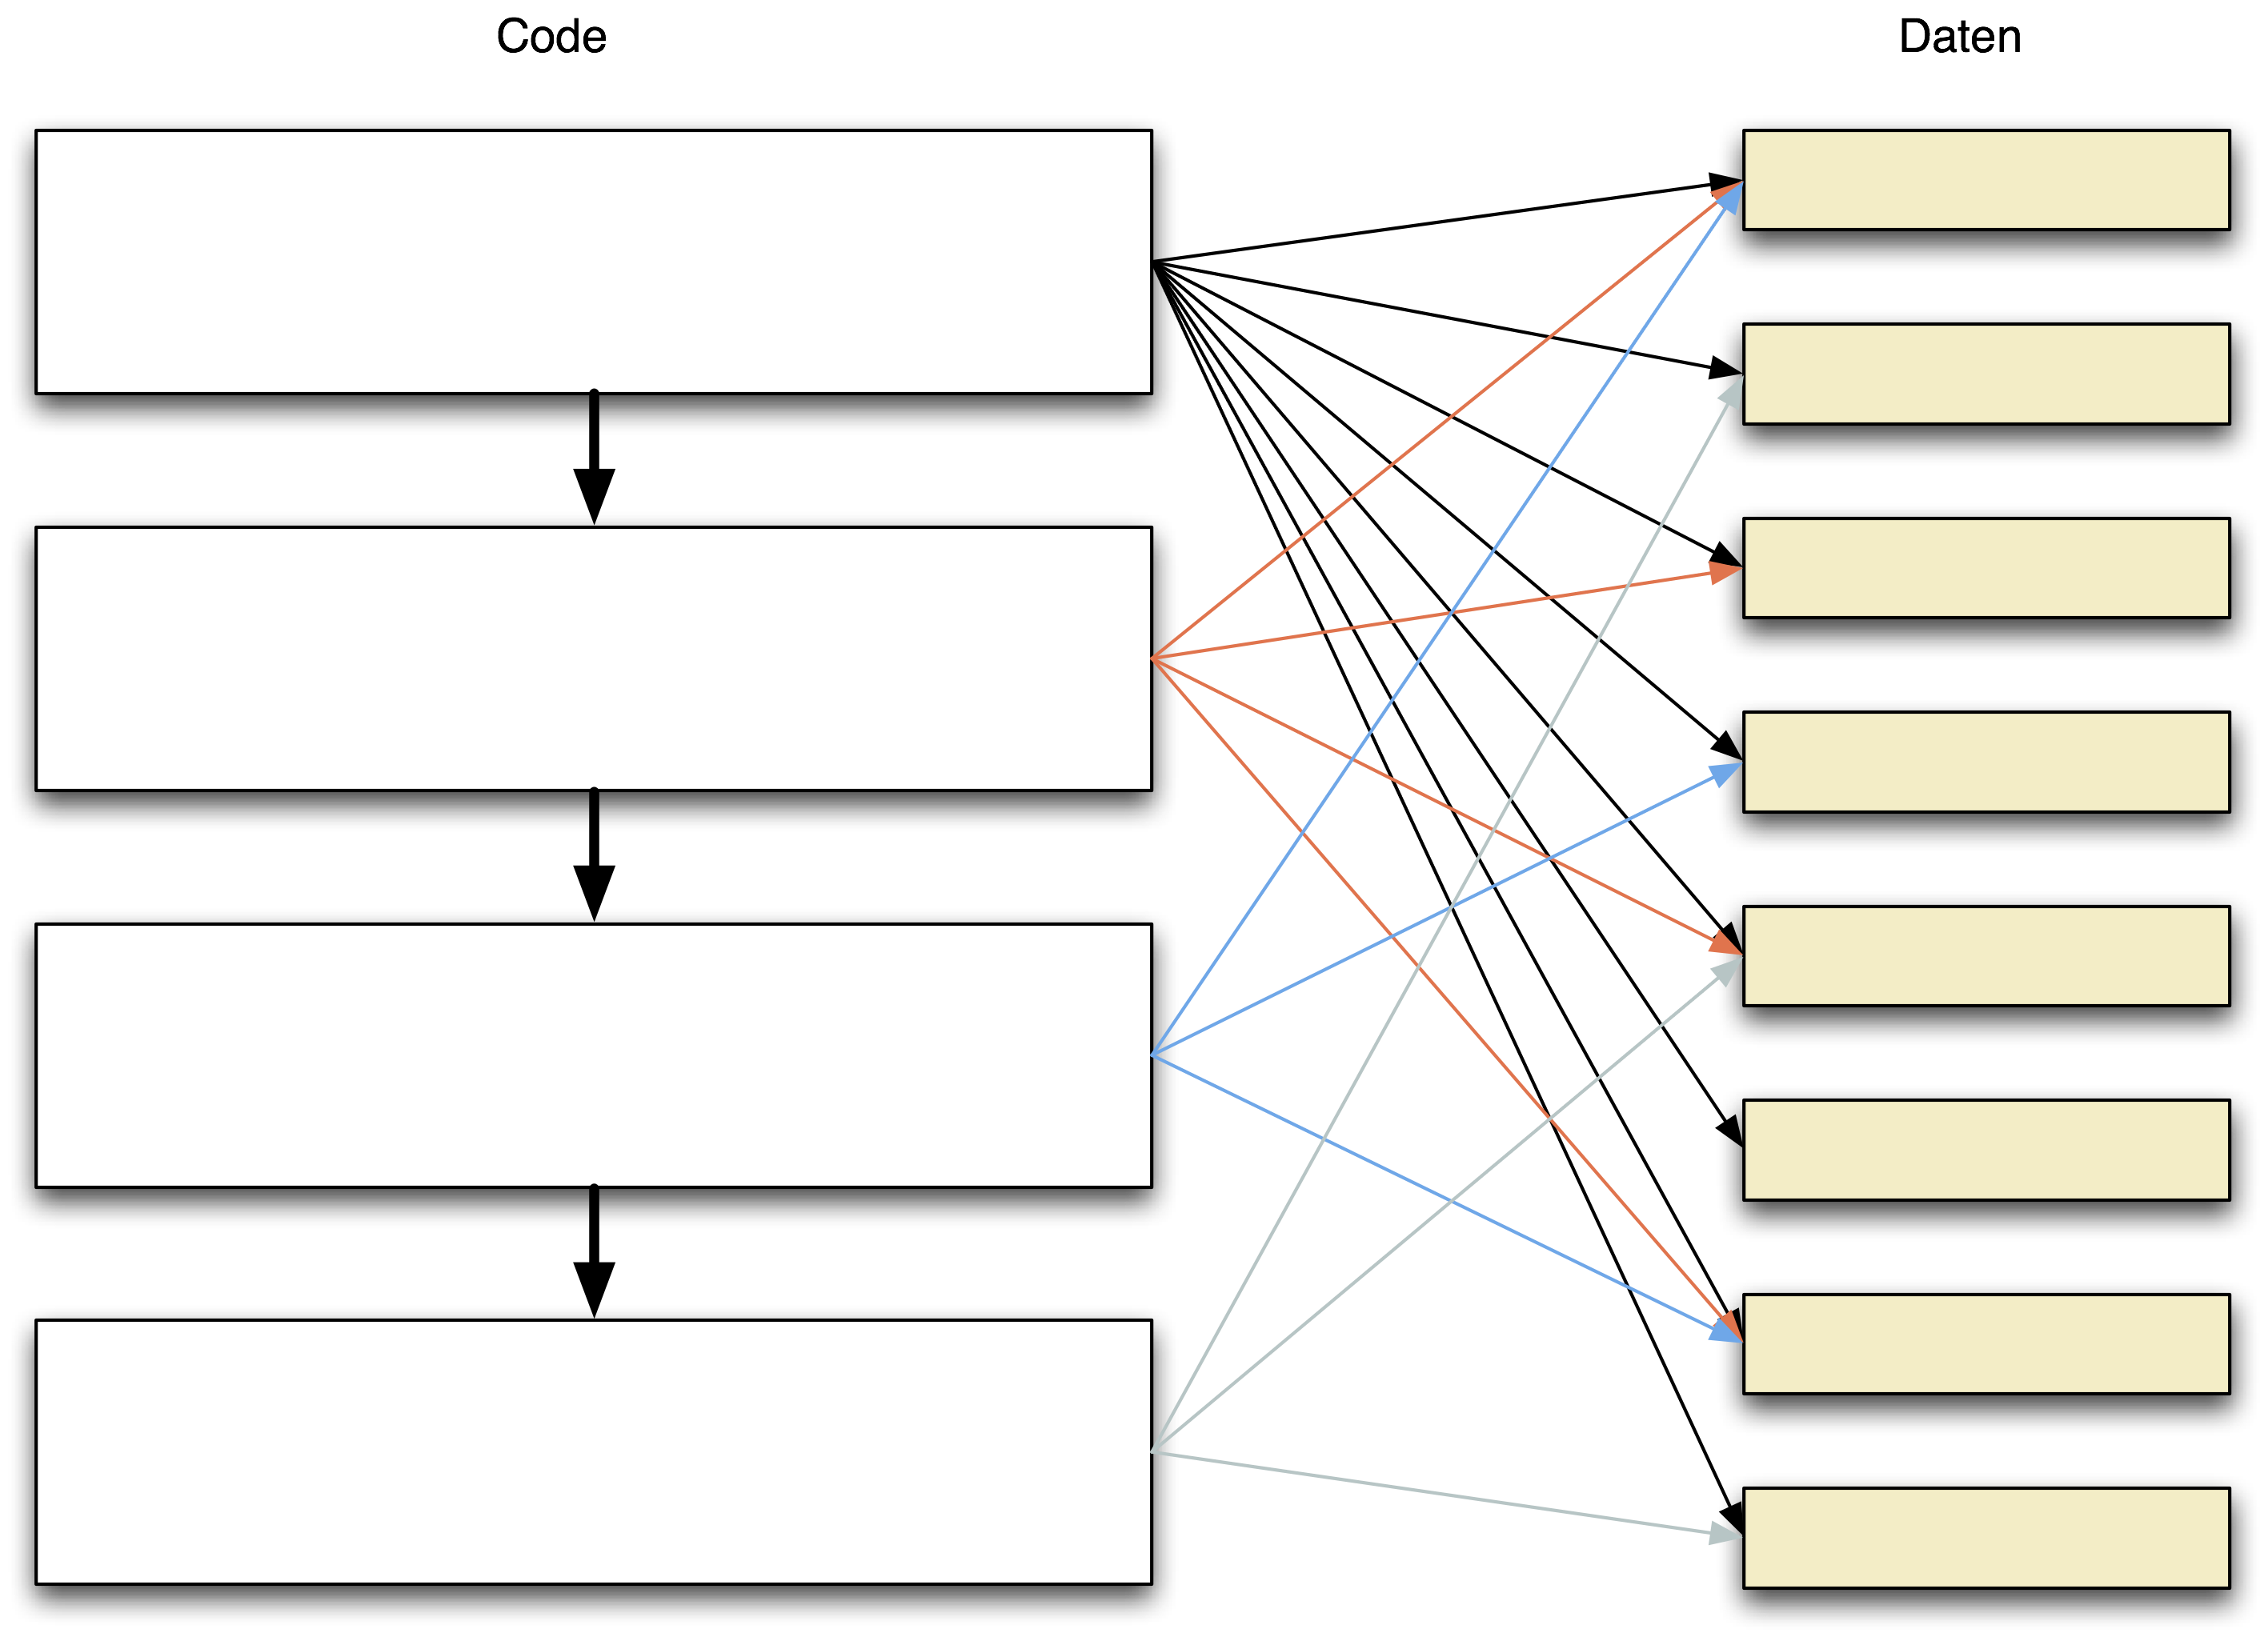
\includegraphics[width=.8 \paperwidth]{Codestruktur.png}
\end{frame}



\begin{frame}[t,fragile]{Vorgehensweise}
\begin{itemize}
\item Fachlich motivierter struktureller Umbau
\item Push-Strukturen in Pull-Strukturen umwandeln
\end{itemize}
\end{frame}

\begin{frame}[t,fragile]{Der erste Ansatz}
\begin{itemize}
\item Unser größter Fehler: Aufbau der Zielstruktur und Neuimplementierung der Logik anhand einer vom Code unabhängigen Spezifikation
\end{itemize}
$\Longrightarrow$ Viele Abweichungen in den Ergebnissen, lange Phase der fachlichen Klärung
\end{frame}

\begin{frame}[t,fragile]{}
\begin{itemize}
\item
\end{itemize}
\end{frame}

\begin{frame}[t,fragile]{}
\begin{itemize}
\item
\end{itemize}
\end{frame}

\begin{frame}[t,fragile]{}
\begin{itemize}
\item
\end{itemize}
\end{frame}

\begin{frame}[t,fragile]{}
\begin{itemize}
\item
\end{itemize}
\end{frame}

\begin{frame}[t,fragile]{}
\begin{itemize}
\item
\end{itemize}
\end{frame}

\begin{frame}[t,fragile]{Der zweite Ansatz}
\begin{itemize}
\item Umbau unter größtmöglicher Weiterverwendung der bereits implementierten Logik
\item Codeveränderungen betreffen lediglich die Struktur
\end{itemize}
\end{frame}

\begin{frame}[t,fragile]{Umbau: Vorbereitung}
\begin{itemize}
\item Existierenden Code duplizieren
\item Feature Toggle an den Aufrufstellen
\end{itemize}
\end{frame}
 
\begin{frame}[t,fragile]{Vorarbeiten}
\begin{itemize}
\item Java-Datumsarithmetik kapseln, z.~B.
\begin{itemize}
\item Joda Time
\item Eigene Klassen
\end{itemize}
\item Namensgebung von Variablen verbessern
\end{itemize}
\end{frame}

\begin{frame}[t,fragile]{Aspekte isolieren}
\begin{itemize}
\item Inline method: Nur noch eine Methode
\item Pro Ergebniswert ein Duplikat dieser Methode
\item Jeweils Irrelevantes aus den Methoden entfernen
\end{itemize}
\end{frame}

\begin{frame}[t,fragile]{Strukturellen Code isolieren}
\begin{itemize}
\item Schleifen über Ergebnisstruktur nach außen bringen
\item Schleifen vereinheitlichen
\end{itemize}
\end{frame}

\begin{frame}[t,fragile]{Zielstruktur aufbauen}
\begin{itemize}
\item Zuerst nur als Gerüst mit Befüllung von außen
\item Berechnung \textbf{eines} Werts in die Zielstruktur übertragen
\item Prüfen der Tragfähigkeit der Zielstruktur
\end{itemize}
\end{frame}

\begin{frame}[t,fragile]{Vervollständigung}
\begin{itemize}
\item Wert für Wert in die Zielstruktur übertragen
\item Parallel dazu Unit-Tests aufbauen
\item Refactoring: 
\begin{itemize}
\item Extrahieren von Methoden
\item Zusammenfassen gleicher Funktionalität
\item Generelle Aufräumarbeiten
\end{itemize}
\item Klärung fachlicher Unklarheiten, Korrektur der Logik
\end{itemize}
\end{frame}

\begin{frame}[t,fragile]{}
\begin{itemize}
\item
\end{itemize}
\end{frame}

\begin{frame}[t,fragile]{}
\begin{itemize}
\item
\end{itemize}
\end{frame}

\begin{frame}[t,fragile]{}
\begin{itemize}
\item
\end{itemize}
\end{frame}

\begin{frame}[t,fragile]{}
\begin{itemize}
\item
\end{itemize}
\end{frame}

\begin{frame}[t,fragile]{}
\begin{itemize}
\item
\end{itemize}
\end{frame}

